% =============================================================================
% Global SOC Mean Transit Time --- SUPPLEMENTARY INFORMATION (for main_Nature)
% =============================================================================
% Companion to main_Nature.tex. Contains the DETAILED methods (the online Methods
% in the article is the concise version) plus the Supplementary Figures/Tables that
% do not fit the 10-item Extended Data budget. Reuses the same references.bib and
% the same figure files as the article. This is a SEPARATE root document: set it as
% the main document in Overleaf to compile it.
% =============================================================================

\documentclass[12pt, a4paper]{article}

\usepackage[utf8]{inputenc}
\usepackage[T1]{fontenc}
\usepackage{geometry}
\usepackage{setspace}
\usepackage{natbib}
\usepackage{graphicx}
\usepackage{float}
\usepackage{amsmath}
\usepackage{booktabs}
\usepackage{tabularx}
\usepackage{multirow}
\usepackage{hyperref}
\usepackage{xcolor}
\usepackage{caption}
\captionsetup{font=small, labelfont=bf, textfont=it}
\newcommand{\PH}[1]{\textcolor{red}{#1}}

\hypersetup{colorlinks=true, linkcolor=black, citecolor=blue!60!black, urlcolor=blue!60!black}
\geometry{margin=2.5cm}
\onehalfspacing

% Supplementary numbering: S1, S2, ...
\renewcommand{\thefigure}{S\arabic{figure}}
\renewcommand{\thetable}{S\arabic{table}}
\renewcommand{\theequation}{S\arabic{equation}}
\renewcommand{\thesection}{S\arabic{section}}

\title{Supplementary Information\\[4pt]
\large Beyond climate: the zonality of soil organic carbon transit times}
\date{}

\begin{document}
\maketitle

\tableofcontents
\newpage

% =============================================================================
\section{Supplementary Methods}
% =============================================================================
% Full procedural detail. The article's online Methods is the concise summary;
% this is the authoritative long version.

\subsection{Conceptual framework}
We define the mean transit time ($\tau$) of SOC as the average time a carbon atom
spends in the soil from entry to exit \citep{Sierra2017,Sierra2018}. Under
steady-state assumptions (constant SOC stock and input flux) and a single homogeneous
pool, $\tau$ equals the ratio of the SOC stock to the annual carbon input flux and is
the inverse of the apparent first-order decomposition rate constant $k$
(Eq.~\ref{eq:mtt_si}). For multi-pool systems, $\tau$ as computed here is a bulk
diagnostic that aggregates pools with different turnover rates \citep{Sierra2018};
this metric is widely used as a first-order characterisation of SOC dynamics and is
directly comparable to the transit-time diagnostics computed from ESM output
\citep{Carvalhais2014,Sierra2017}.
\begin{equation}
  \tau \;=\; \frac{\text{SOC}_\text{stock}}{C_\text{input}} \;=\; \frac{1}{k}
  \label{eq:mtt_si}
\end{equation}

\subsection{Soil data compilation}
Soil profile data were compiled from the OpenLandMap Open Compendium of Soil Datasets
\citep{OpenLandMapSoilDB2025} (\texttt{sol\_chem.pnts\_horizons}), a harmonised global
collection integrating observations from many national and regional soil surveys. From
the horizon-level records we retained only mineral soils by removing records with
organic carbon (OC) $\geq120$~g\,kg$^{-1}$. Horizon-level measurements of seven
variables (organic carbon, total nitrogen, pH~(H$_2$O), clay, silt, sand, and oven-dry
bulk density) were standardised to 0--20~cm by thickness-weighted averaging, applied to
each profile individually. Site-level metadata (coordinates, observation date, source
database) were carried forward as the most common value across horizons.

\subsection{Data quality control}
After depth standardisation the dataset contained 381{,}541 profiles from 47 source
databases (78\textdegree S--78\textdegree N). We then removed records likely to bias the
transit-time calculation: OC~$=$~0 values that encode missing data in these sources
(83{,}206 profiles, 21.8\,\%) were set to \texttt{NA}; 102{,}379 exact duplicates
(matching coordinates and OC; 26.8\,\%) were removed; bulk-density values outside
0.1--2.5~g\,cm$^{-3}$ were set to \texttt{NA}. After filtering, 198{,}382 profiles
remained (52.0\,\%). Profiles with integer-only coordinates ($n=208$) and unusually
high OC ($>100$~g\,kg$^{-1}$; $n=3{,}252$) were flagged but retained.

\subsection{Bulk density gap-filling}
Bulk density (BD) is required to convert OC concentration to SOC stock but is
frequently unreported. We used a three-tier approach. First, a Random Forest
(\texttt{randomForest}; 200 trees) was trained on profiles with measured BD, using
terrain metrics, K\"oppen zone, land-cover fractions, SoilGrids 250\,m v2.0 properties
\citep{Poggio2021} (excluding BD), MODIS NPP, WRB functional group, and MODIS burn
count. Ten-fold cross-validation confirmed the RF outperformed the SoilGrids BD
product. Second, profiles lacking measured BD but with complete RF predictors received
RF predictions. Third, remaining gaps were filled with the SoilGrids BD product. Each
profile was flagged with its BD source.

\subsection{Mean transit time calculation}
SOC stock for 0--20~cm was
\begin{equation}
  \text{SOC}_\text{stock}\;[\text{g\,C\,m}^{-2}] \;=\; \text{OC}\times\text{BD}\times20\times10,
  \label{eq:soc_stock_si}
\end{equation}
with OC in g\,kg$^{-1}$, BD in g\,cm$^{-3}$, depth in cm, and the factor 10 reconciling
units. Carbon input was estimated as the belowground fraction of net primary
productivity (BNPP). Root-derived carbon is preferentially stabilised in persistent SOC
\PH{[cite: Rasse 2005; Jackson 2017]}, so the belowground fraction is a deliberate,
conservative boundary for the input flux; sensitivity to this choice (including
aboveground litter and forest harvest) is examined in
Sec.~\ref{sec:si_robust}. We used MODIS MOD17A3 annual NPP
\citep[2001--2020;][]{Running2015}, applying the MODIS scale factor and using only
NPP years preceding each site's sampling date. Belowground allocation fractions were
assigned by dominant land cover following \citet{Mokany2006}, \citet{Malhi2011}, and
\citet{Litton2008} (Table~\ref{stab:allocation}):
\begin{equation}
  C_\text{input}\;[\text{g\,C\,m}^{-2}\text{\,yr}^{-1}] \;=\; \text{NPP}\times f_\text{BNPP}^{(\text{lc})},
  \label{eq:c_input_si}
\end{equation}
and $\tau$ followed from Eq.~\ref{eq:mtt_si}. Values with $\tau<1$ or $>1000$~yr, or
missing/negative/infinite, were excluded, and the upper and lower 1\,\% tails removed
before fitting.

\subsection{Predictor variables}
Predictors were organised into four mechanistically distinct groups (Extended Data
Table~1 of the article).
\emph{Climate}: ERA5-Land monthly means \citep[2001--2020;][]{MunozSabater2021} reduced
to mean 2-m temperature, temperature seasonality, depth-weighted soil temperature and
moisture (weights 0.35/0.65 for layers 1/2), snow cover, and potential evaporation;
plus the 30-class K\"oppen--Geiger classification of \citet{Beck2023} resampled to
$0.1\textdegree$ by mode.
\emph{Edaphic}: SoilGrids 250\,m v2.0 \citep{Poggio2021} depth-weighted to 0--20~cm
(clay, sand, bulk density, coarse fragments, pH, CEC, nitrogen), converted from integer
encoding with published \texttt{d\_factor} divisors identically at points and grids;
terrain metrics from the Copernicus GLO-30 DEM \citep{CopernicusDEM2022}; and a WRB Most
Probable class \citep{Poggio2021} reclassified into eight mechanistic functional groups
(sandy/coarse, temperate agricultural, high-clay tropical, arid/chemical, poorly
drained, volcanic, shallow/young, cold/permafrost).
\emph{Land use and disturbance}: ESA WorldCover 2021 \citep{Zanaga2022} fractional
covers (six used as predictors); forest-loss year from Hansen GFC v1.10
\citep{Hansen2013} as a pre-sampling binary; and cumulative pre-sampling burn count
from MODIS MCD64A1 \citep[2001--2020;][]{Giglio2018}. Only disturbance predating each
sample is retained, for consistency with the steady-state framing.
\emph{Biological}: global fungal proportion \citep{Yu2022}; AM/EcM root colonisation and
their ratio \citep{Barcelo2023}; and mycorrhizal richness and endemism from the SPUN
Global Underground Atlas \citep{VanNuland2025}. Six of these nine layers form the
default set used throughout ($\geq96\,\%$ coverage); the three \citet{Barcelo2023}
root-colonisation layers sharply reduce coverage (${\sim}61\,\%$) while adding
negligible unique skill and enter only the nine-layer sensitivity
(Sec.~\ref{sec:si_robust}).
All covariates were resampled to a common $0.1\textdegree$ ($\sim$11~km) WGS84 grid
(set by the coarsest, climatic, layers), continuous by bilinear interpolation and
categorical by mode.

\subsection{Modelling design and attribution}
Productivity variables (NPP, LAI) are excluded by design: because $\tau$ is SOC stock
divided by an NPP-derived input (Eq.~\ref{eq:mtt_si}), admitting productivity would make
the model circular. Because the groups are spatially correlated (climate is itself a
soil-forming factor), explained variance cannot be attributed by adding groups one at a
time; we therefore use an order-independent Shapley decomposition
(Sec.~\ref{sec:si_shapley}), and separately test whether the beyond-climate residual is
organised (Sec.~\ref{sec:si_moran}), where it acts (Sec.~\ref{sec:si_map}), and how each
driver acts (Sec.~\ref{sec:si_ale}). Nested configurations are labelled M1 (Climate)
through M7 (full model); unless noted every model uses the six-layer biological set.

\subsection{Random Forest fitting and spatial cross-validation}
All models were fitted with \texttt{ranger} \citep{Wright2017} (500 trees, minimum node
size 5, $m_\text{try}=\lfloor\sqrt{p}\rfloor$) on $\ln\tau$. Predictive performance is
the spatially cross-validated $R^2$, estimated by partitioning the globe into
$2\textdegree$ ($\sim$200~km) blocks, assigning blocks to ten folds, and predicting each
fold from a model trained on the other nine. Holding out whole blocks prevents a site
near a fold boundary from being predicted by an almost-coincident training neighbour, so
the reported $R^2$ measures generalisation to unseen regions. The $2\textdegree$ block is
far wider than the residual's correlation range ($\approx16$~km;
Sec.~\ref{sec:si_map}). The attribution is insensitive to block size: repeating the
decomposition at $1\textdegree$ and $5\textdegree$ shifts each group's share by at most
2 percentage points, leaving the ranking and the climate-versus-non-climate split
unchanged (Fig.~\ref{sfig:blocksize}).

\subsection{Attribution of variance among process classes (Shapley)}
\label{sec:si_shapley}
Let $N$ be the four groups and $v(S)$ the spatially cross-validated $R^2$ of the model
fitted on subset $S\subseteq N$. We fit all $2^4=16$ subsets on a common row set
($n=154{,}675$ complete across all groups) so every $v(S)$ is comparable. The Shapley
value of group $i$ is
\begin{equation}
  \phi_i = \!\!\sum_{S\subseteq N\setminus\{i\}}
  \frac{|S|!\,(|N|-|S|-1)!}{|N|!}\,[\,v(S\cup\{i\})-v(S)\,],
  \label{eq:shapley_si}
\end{equation}
the order-averaged marginal contribution; the $\phi_i$ sum to the full-model
$R^2=v(N)$ and are reported as percentage shares. Alongside them we report each group's
single-domain skill $v(\{i\})$: the two are complementary (total signal versus unique
contribution), and their overlap $\sum_i v(\{i\})-v(N)$ quantifies how much the groups'
contributions coincide, an expression of the zonal coupling between climate and soil
rather than a defect. The three root-colonisation layers add negligible unique skill
($\Delta R^2\approx0.001$) while cutting biological coverage from $\geq96\,\%$ to
$61\,\%$, so they enter only the nine-layer sensitivity (Fig.~\ref{sfig:parsimony}).

\subsection{Spatial organisation of the beyond-climate residual (Moran's $I$)}
\label{sec:si_moran}
We take the beyond-climate residual as the out-of-sample $\ln\tau$ minus the
climate-only prediction, aggregate it to block means, and compute
\begin{equation}
  I=\frac{n}{\sum_{ij}w_{ij}}\cdot
  \frac{\sum_{ij}w_{ij}(x_i-\bar x)(x_j-\bar x)}{\sum_i (x_i-\bar x)^2},
  \label{eq:moran_si}
\end{equation}
where the spatial lag is each block's average over its eight nearest neighbouring blocks
(row-standardised $k=8$ weights). Significance is assessed against 999 random spatial
permutations. We evaluate $I$ at $2\textdegree$ and $5\textdegree$ aggregation (with
$k=8$ held fixed).

\subsection{Mapping the zonality, and choosing the scale}
\label{sec:si_map}
The modulation field is the log-ratio of model predictions
$\ln[\hat\tau_\text{context}/\hat\tau_\text{climate}]$, computed symmetrically (each
domain relative to climate) to match the order-independent attribution; abiotic and
biological panels are shown separately. From the same fields we derive a discrete
zonation: at each $2\textdegree$ block we weight each domain's log-ratio by its Shapley
share and label the block by the largest, or as "climate alone" where none exceeds a
small threshold. The noise floor is characterised by the residual variogram
(nugget/sill $\approx0.56$, range $\approx16$~km); this range reflects the effective
resolution of the gridded predictor stack (MODIS NPP, climate reanalysis, SoilGrids),
which are smooth at hundreds of metres to kilometres, not intrinsic soil
autocorrelation. The mapping scale is set by an out-of-sample skill curve: agreement
between the mapped and observed residual rises from $\approx0.11$ at the native pixel to
$\approx0.22$ at 1--2\textdegree{} and is flat across 1--7\textdegree{}
(Fig.~\ref{sfig:mapskill}); a purely linear version declines with scale, so the
meso-scale choice rests on the nonlinear, map-faithful metric. We map at $2\textdegree$.

\subsection{Mechanism: marginal responses (ALE)}
\label{sec:si_ale}
We use Accumulated Local Effects \citep{Apley2020} on the full model (M7, six-layer
biology). Each continuous predictor is split into 40 quantile bins; within each bin the
predictor of interest is moved from the lower to the upper edge while all others are held
at their observed values, and the local prediction differences are accumulated and
centred. Working locally, within intervals of co-occurring data, avoids the
extrapolation artefacts that partial-dependence curves suffer under correlation. Curves
are computed globally and within four latitude bands (southern temperate, tropics,
northern temperate, boreal/Arctic; Extended Data Fig.~4 of the article). Categorical
predictors are excluded.

\subsection{Comparison with Earth System Model structure}
We compare the spatial structure of our $\tau$ against six CMIP6 models spanning
structurally distinct land-surface lineages \citep{Varney2022}: CESM2, UKESM1-0-LL,
IPSL-CM6A-LR, MPI-ESM1-2-LR, CanESM5, MIROC-ES2L. For each we computed the
quasi-equilibrium turnover $\tau_\text{ESM}=\text{cSoil}/\text{rh}$
\citep{Koven2017,Carvalhais2014} over 1980--2014 (using \texttt{cSoilAbove1m} for CESM2
to reduce depth mismatch). Absolute turnover is not comparable across products (depth,
pool definition, and reference period differ), so we normalise each product to its own
distribution and summarise structure two ways (relative turnover by biome zone and by
continuous latitude band) together with magnitude-free dispersion statistics
(coefficient of variation, 95:5 percentile ratio, SD of $\ln\tau$;
Table~\ref{stab:esm_dispersion}). We quantify latitudinal amplification as the
polar-to-tropical ratio of relative turnover and compare it with the same ratio in the
map estimated here.

\subsection{Robustness checks}
\label{sec:si_robust}
\emph{Provenance.} We tested whether the residual structure could be an artefact of
combining source databases by measuring the between-source share of residual variance
($\eta^2$) and the change in coarse organisation after removing each source's mean
(Sec.~\ref{sec:si_provenance}, Table~\ref{stab:provenance}).
\emph{Biological parsimony.} We compared per-layer coverage, collinearity, and unique
skill to justify the six-layer set (Fig.~\ref{sfig:parsimony}).
\emph{Block-size sensitivity.} We repeated the Shapley decomposition at $1$, $2$, and
$5\textdegree$ blocks (Fig.~\ref{sfig:blocksize}).
\emph{Carbon-input convention.} Because the input is set by a coefficient on one NPP
field (Eq.~\ref{eq:c_input_si}), a spatially uniform change rescales $\tau$ and leaves
every scale-invariant quantity (block-CV $R^2$, Shapley shares, Moran's $I$) unchanged;
only spatial variation of the coefficient, entering through land cover, can move the
attribution. We re-derived $\tau$ under three conventions (belowground, total NPP, and
total minus a generous forest-harvest export on tree-dominant pixels) and re-ran the
decomposition (Extended Data Fig.~3 and Table~2 of the article); the beyond-climate gap,
Moran's $I$, and Shapley shares are essentially unchanged, only the land-use share
responds, and the gap does not fall as the harvest export fraction is swept across
0.2--0.6.
\emph{Peatlands and open water.} Observations on peat in the Global Peatland Map 2.0
\citep{GreifswaldGPM2022} (both tiers; 6{,}922 profiles, 3.5\,\%) are excluded from the
fit, and peat together with open water is masked, not interpreted, on all maps.

\subsection{Software and reproducibility}
Analyses used R ($\geq4.3$) with \texttt{terra}, \texttt{sf}, \texttt{ranger}
\citep{Wright2017}, and \texttt{gstat}. The pipeline is a sequence of numbered scripts;
each reported number and figure regenerates from a named script. Code and intermediate
outputs are archived at \PH{[DOI]}.

% =============================================================================
\section{Provenance control on the beyond-climate signal}
\label{sec:si_provenance}
% =============================================================================
Because the soil compendium aggregates 44 geographically clustered source databases, a
source-specific measurement or laboratory offset could in principle masquerade as
large-scale (zonal) structure. We tested whether the beyond-climate signal (the residual
of the spatial-block cross-validated climate model) is carried by provenance rather than
ecology. Only \textbf{2.4\,\%} of the residual variance lies between source databases
($\eta^2_\text{source}=0.024$, versus $\eta^2=0.067$ for $5\textdegree$ spatial blocks).
Removing each source's mean residual leaves the coarse-scale organisation essentially
intact and the covariate skill on the block-mean residual barely changed
(Table~\ref{stab:provenance}). Because source membership is itself confounded with
geography, this is a conservative (upper-bound) test: the signal that survives source
removal is unambiguously ecological.

% =============================================================================
\section{Supplementary Figures}
% =============================================================================

\begin{figure}[H]\centering
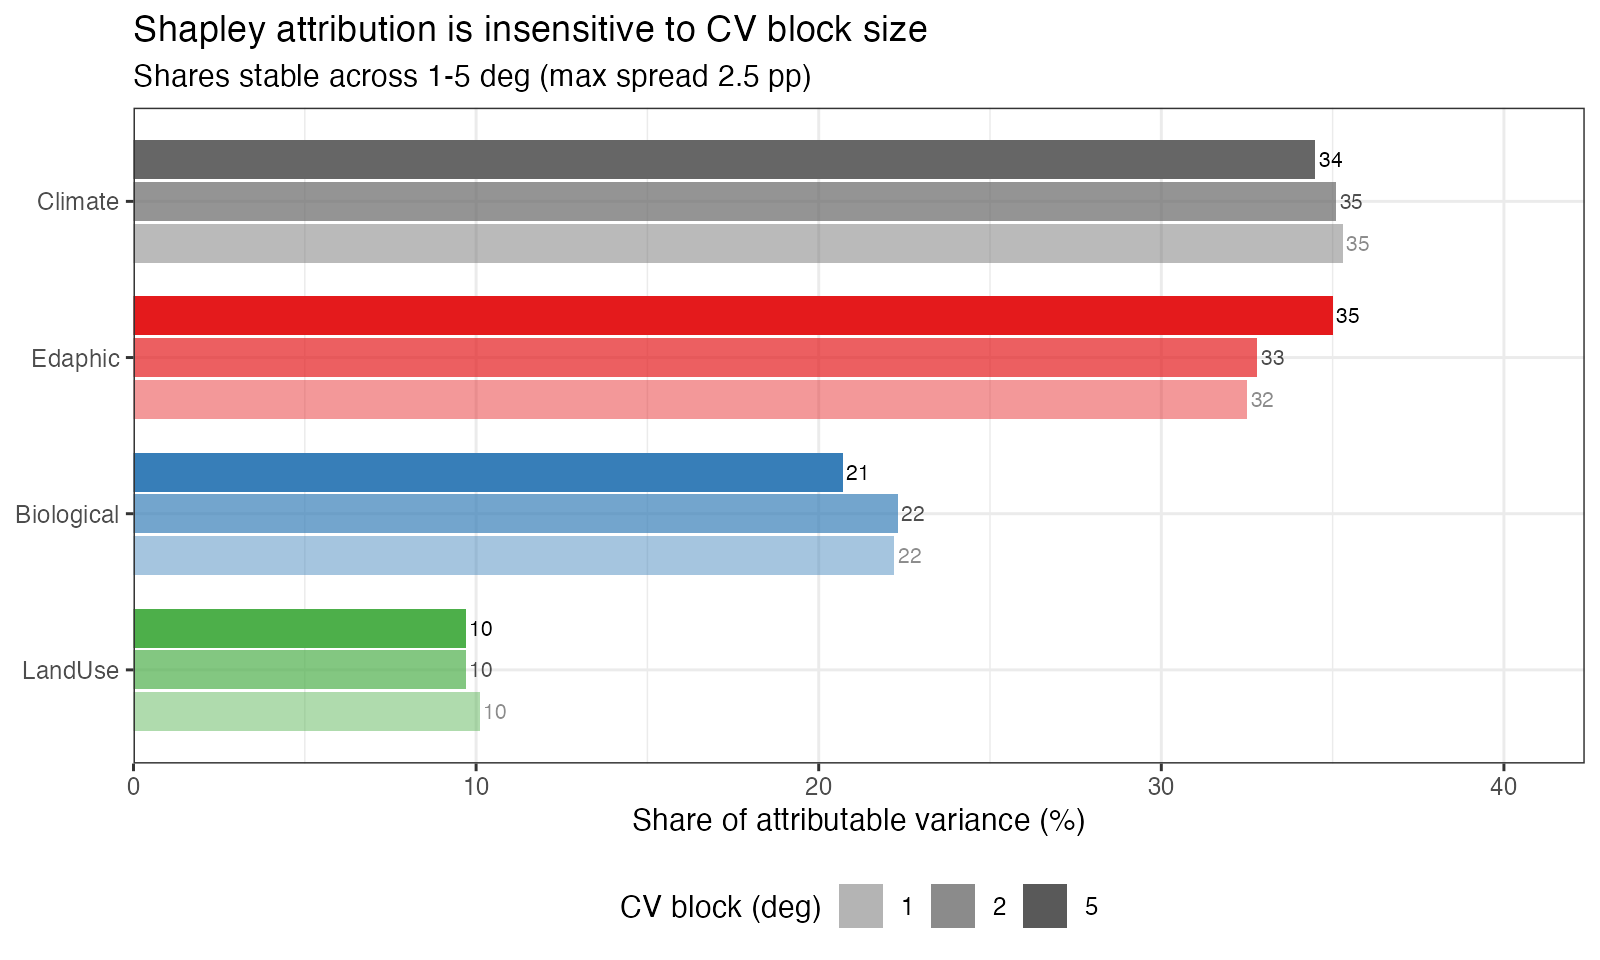
\includegraphics[width=0.8\textwidth]{../plots/step_13c_commonality/13h_blocksize_shapley.png}
\caption{\textbf{Block-size invariance.} Shapley shares across $1/2/5\textdegree$
cross-validation blocks; maximum spread $\le2$~pp.}
\label{sfig:blocksize}
\end{figure}

\begin{figure}[H]\centering
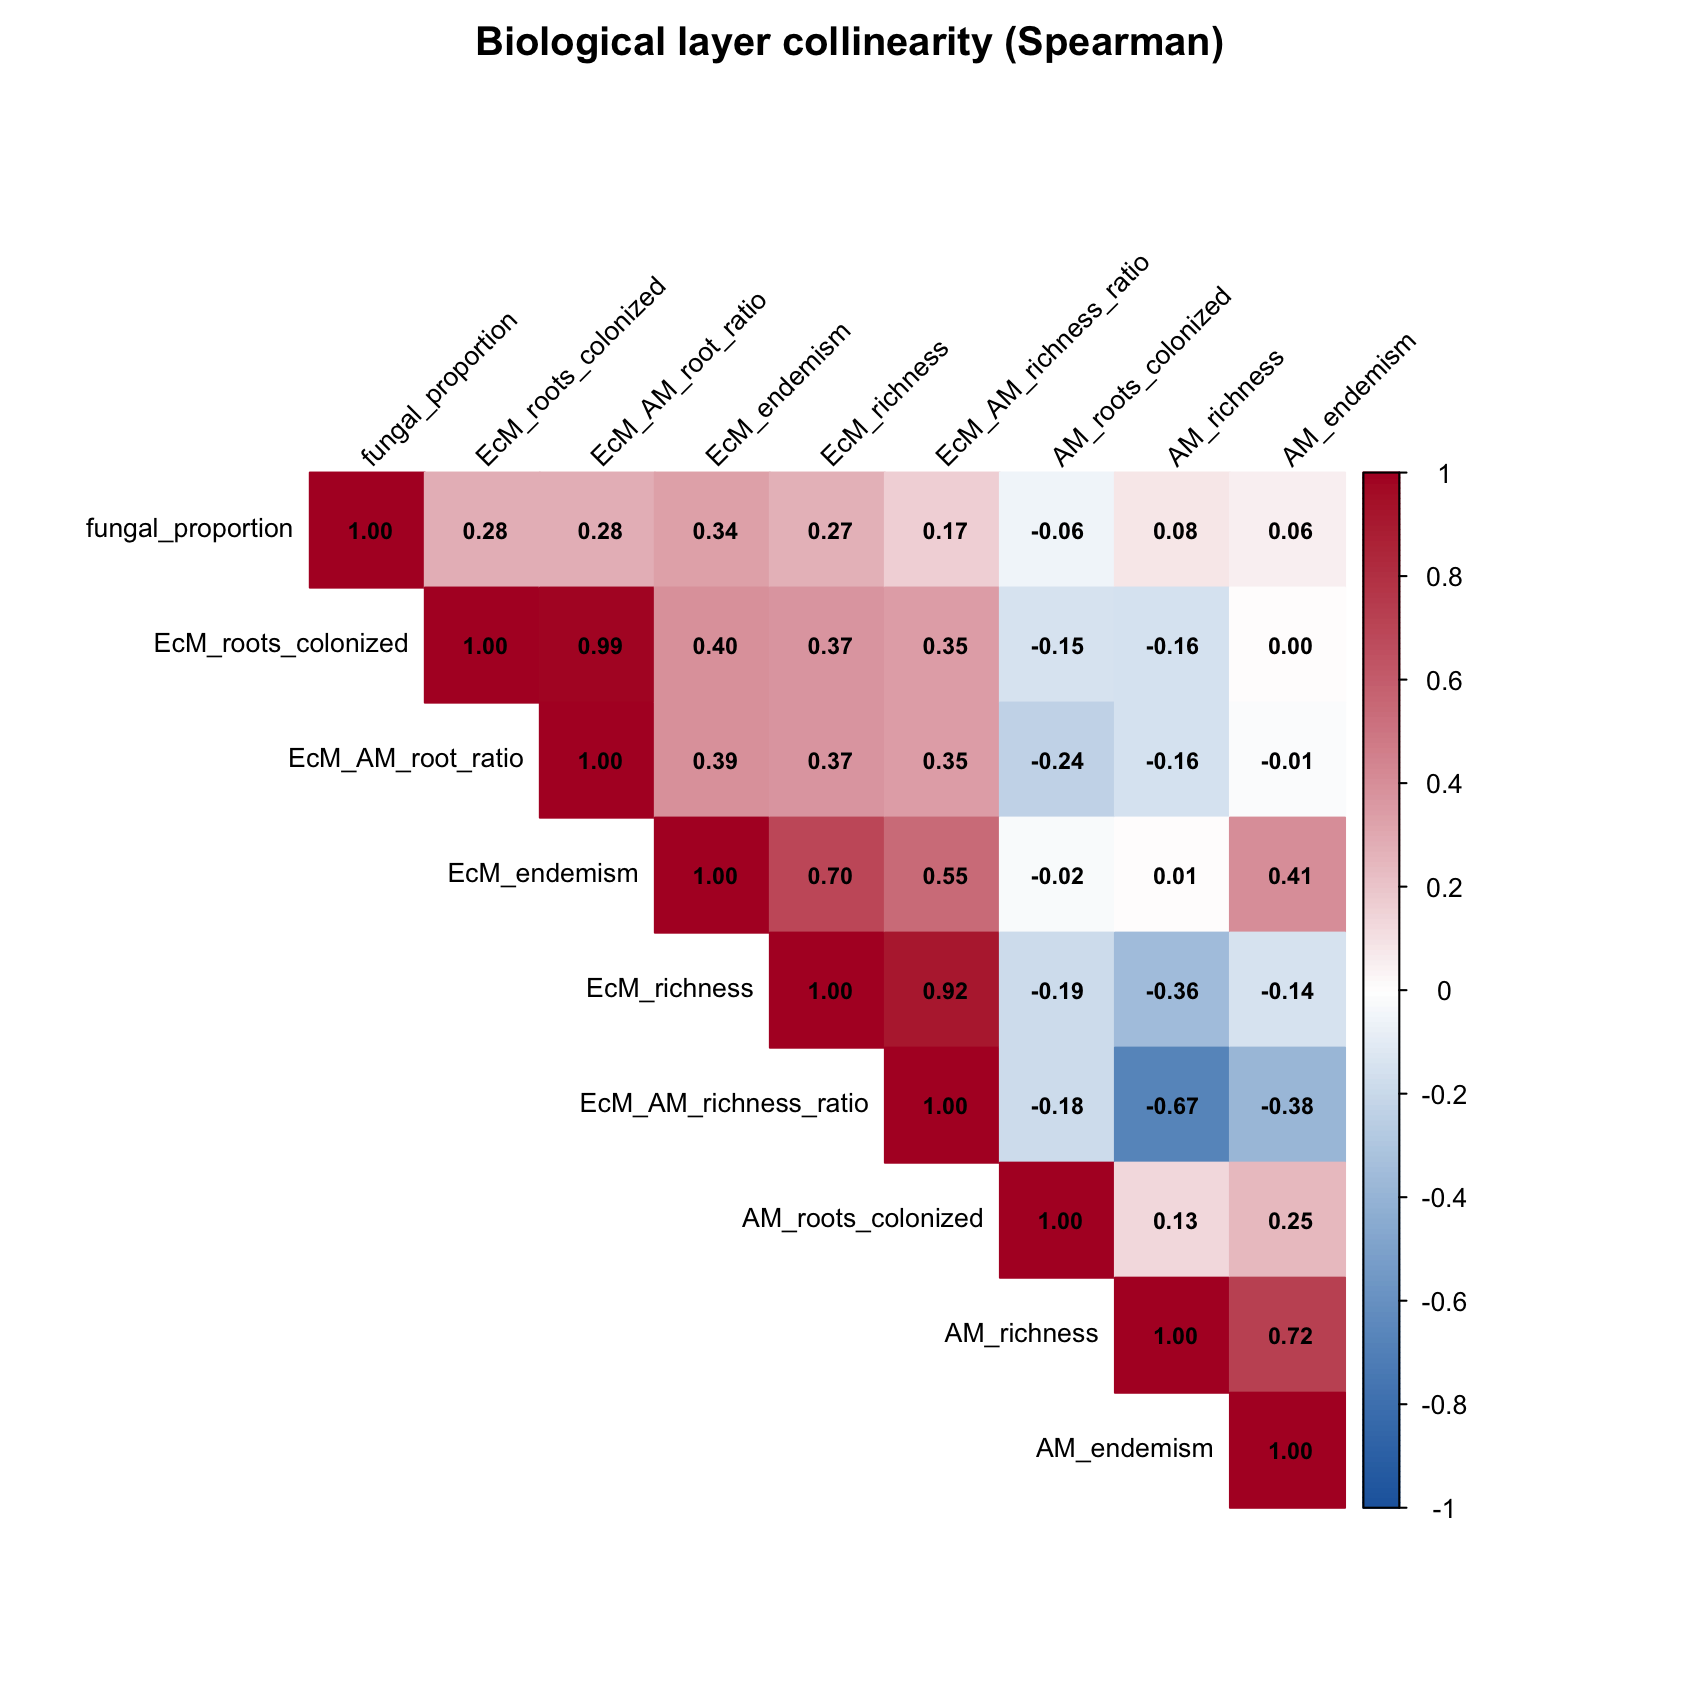
\includegraphics[width=0.95\textwidth]{../plots/appendix/biological_collinearity.png}
\caption{\textbf{Biological parsimony.} Collinearity among the nine biological layers
and single-layer skill versus coverage, justifying the default six-layer set; the three
root-colonisation layers add negligible unique skill.}
\label{sfig:parsimony}
\end{figure}

\begin{figure}[H]\centering
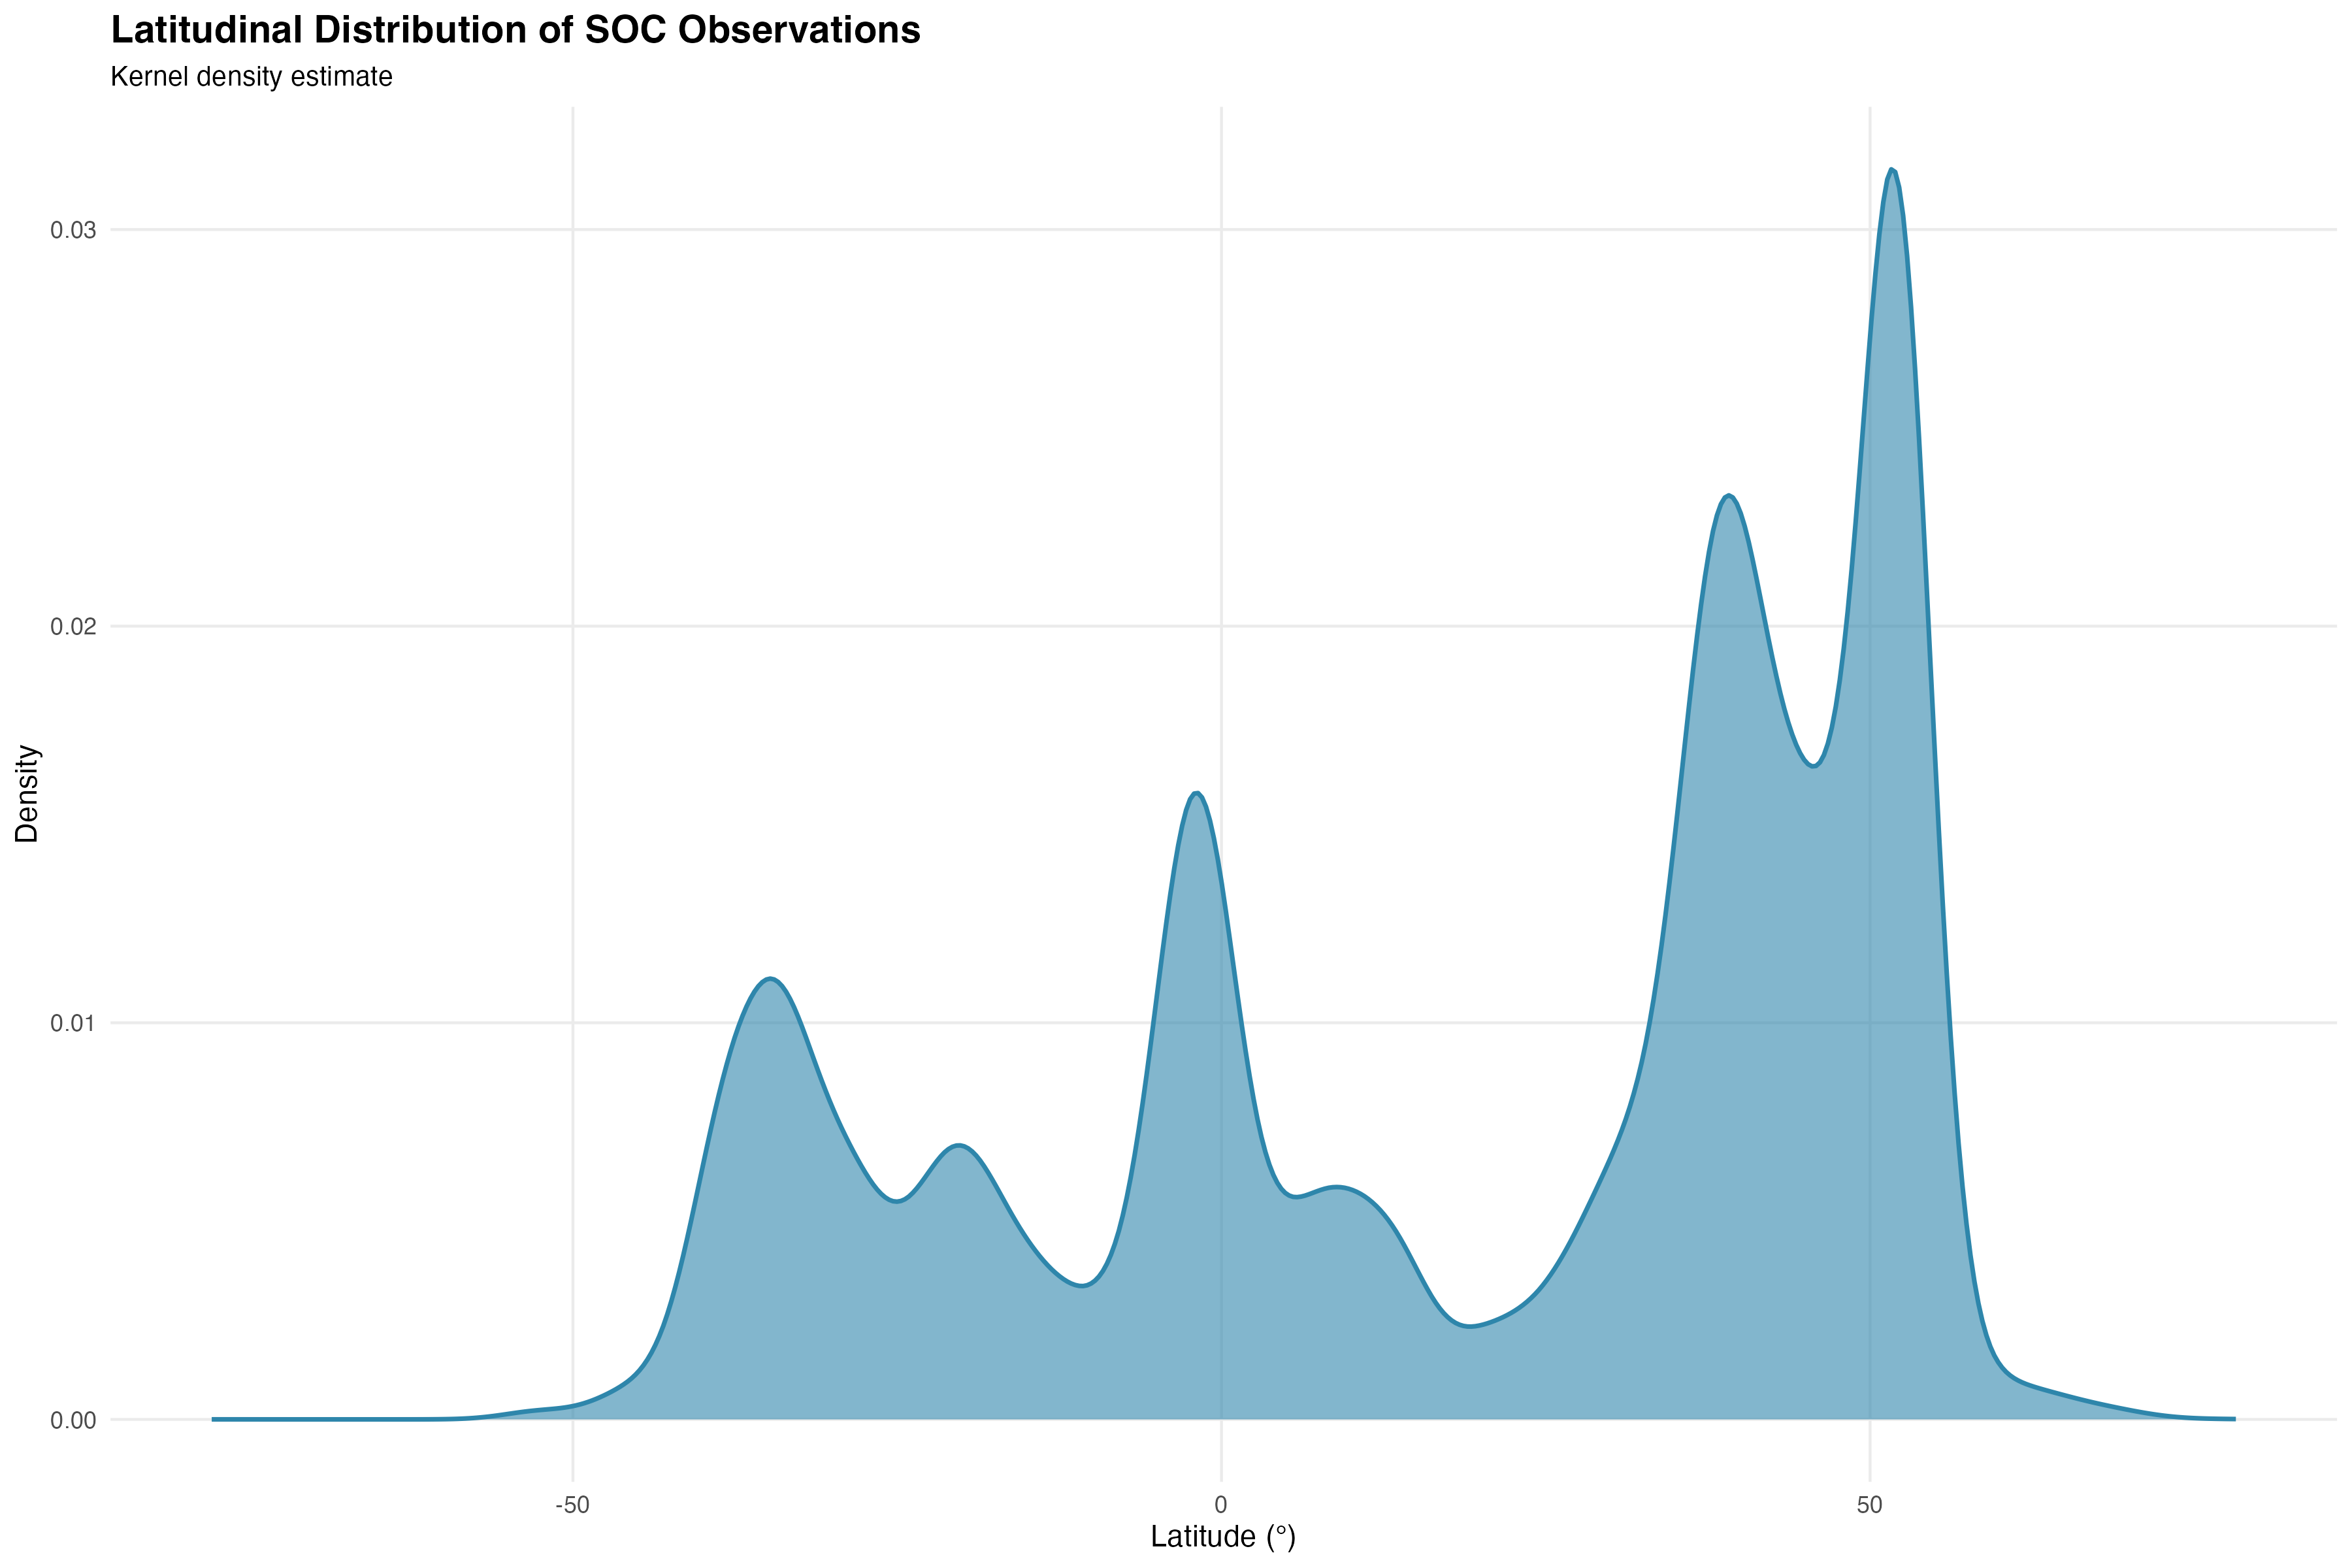
\includegraphics[width=0.95\textwidth]{../plots/step_17_visualizations/latitudinal_sampling_coverage.png}
\caption{\textbf{Latitudinal sampling coverage.} Density of the OpenLandMap soil
profiles used for training, by latitude.}
\label{sfig:sampling}
\end{figure}

\begin{figure}[H]\centering
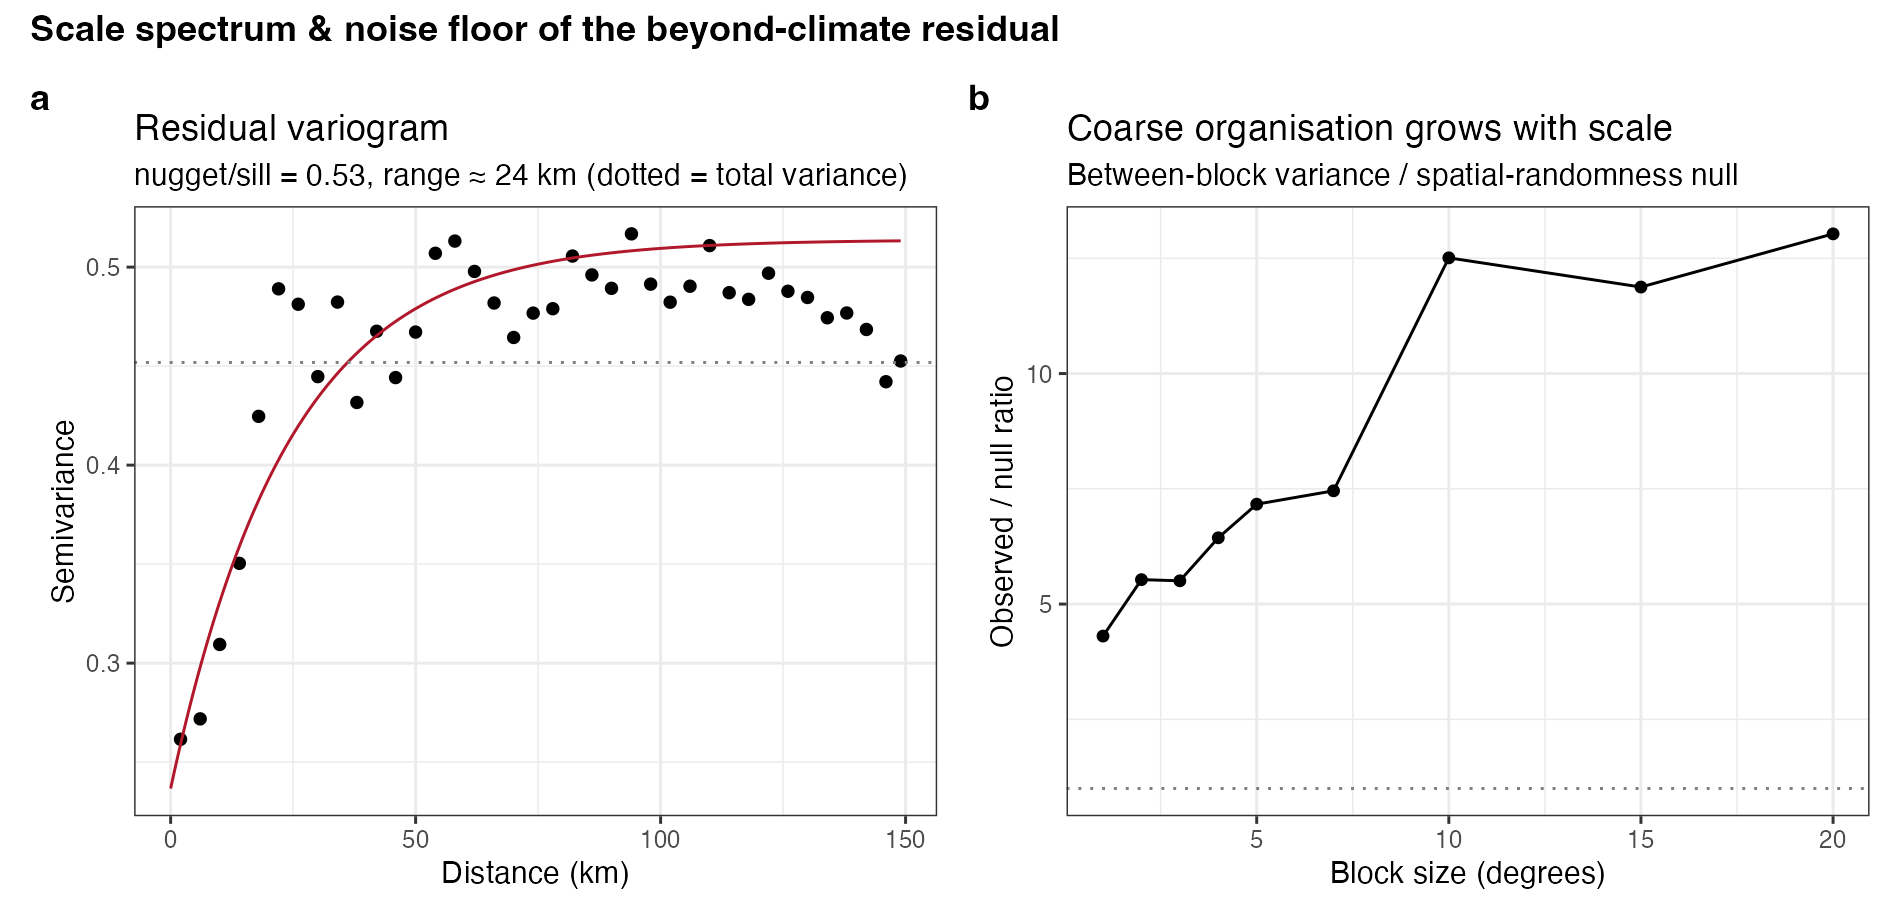
\includegraphics[width=0.95\textwidth]{../plots/appendix/scale_noisefloor.png}
\caption{\textbf{Scale spectrum and noise floor.} (a)~Residual variogram (nugget/sill
$\approx0.56$, range $\approx16$~km); (b)~coarse organisation grows with block size.}
\label{sfig:noisefloor}
\end{figure}

\begin{figure}[H]\centering
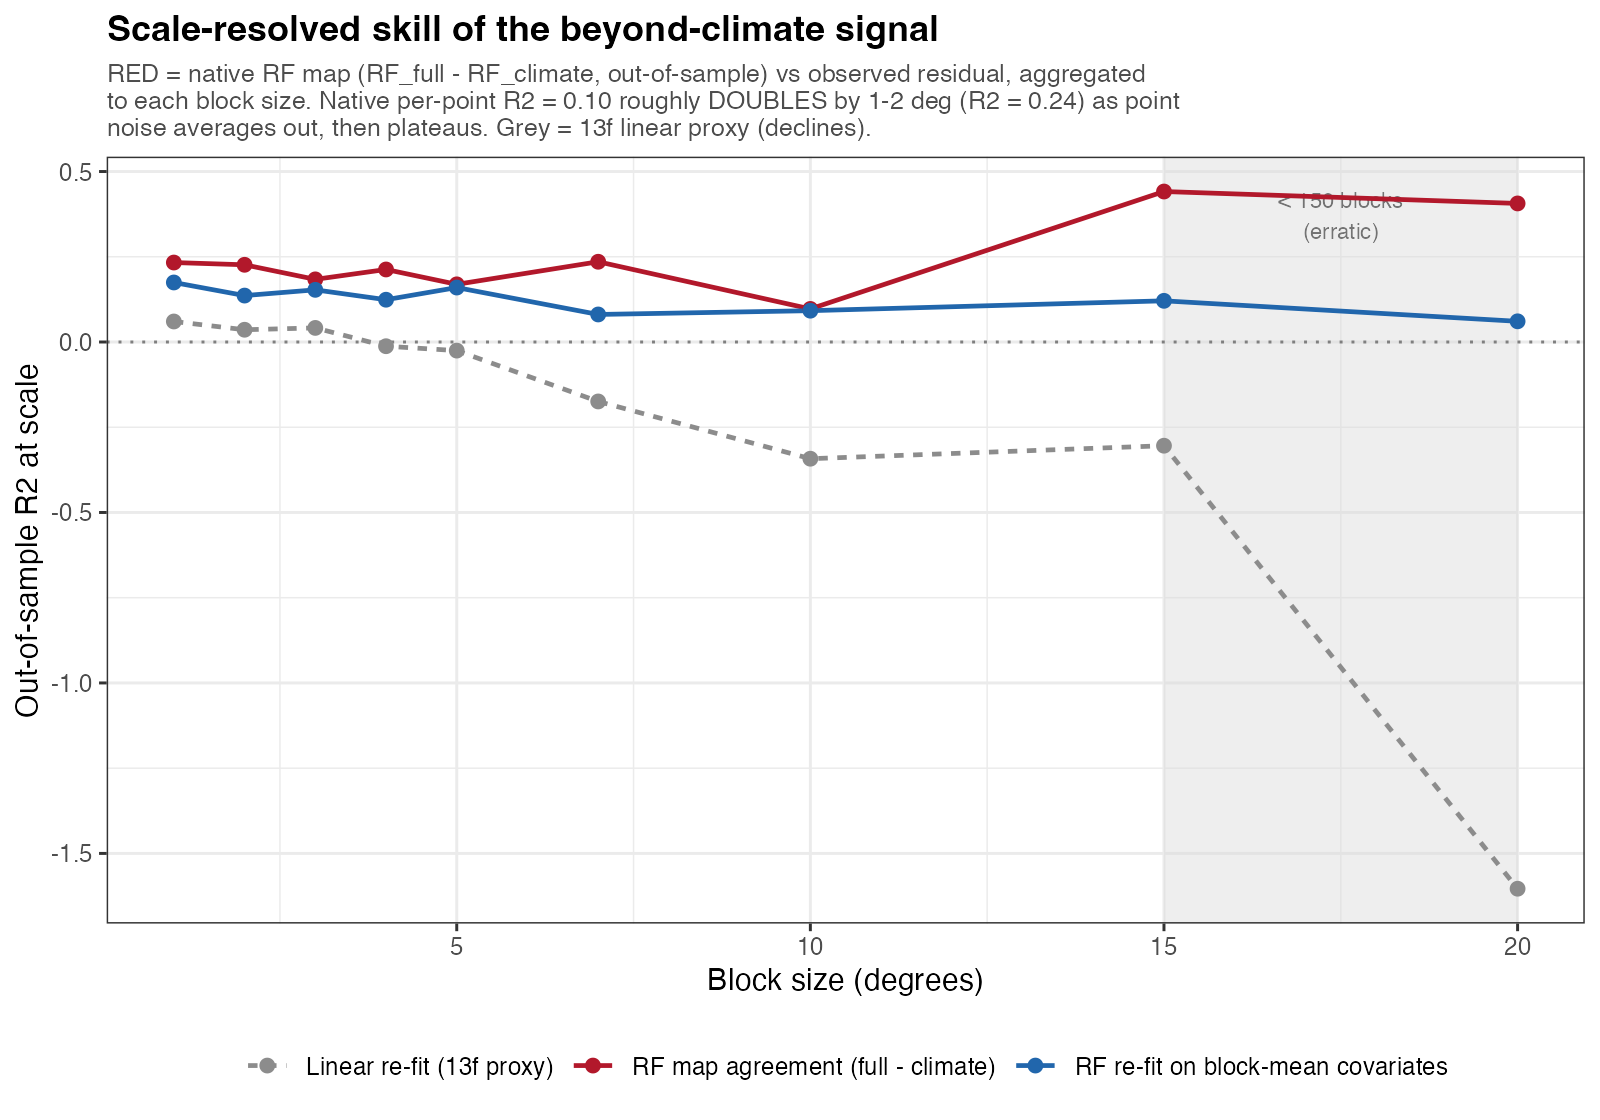
\includegraphics[width=0.85\textwidth]{../plots/appendix/scale_rf_mapping_skill.png}
\caption{\textbf{RF mapping skill versus scale.} Agreement of the native beyond-climate
map with the observed residual when aggregated to each block size: $R^2\approx0.11$
native, $\approx0.22$ by 1--2\textdegree, plateau across 1--7\textdegree; the linear
proxy (grey) declines.}
\label{sfig:mapskill}
\end{figure}

\begin{figure}[H]\centering
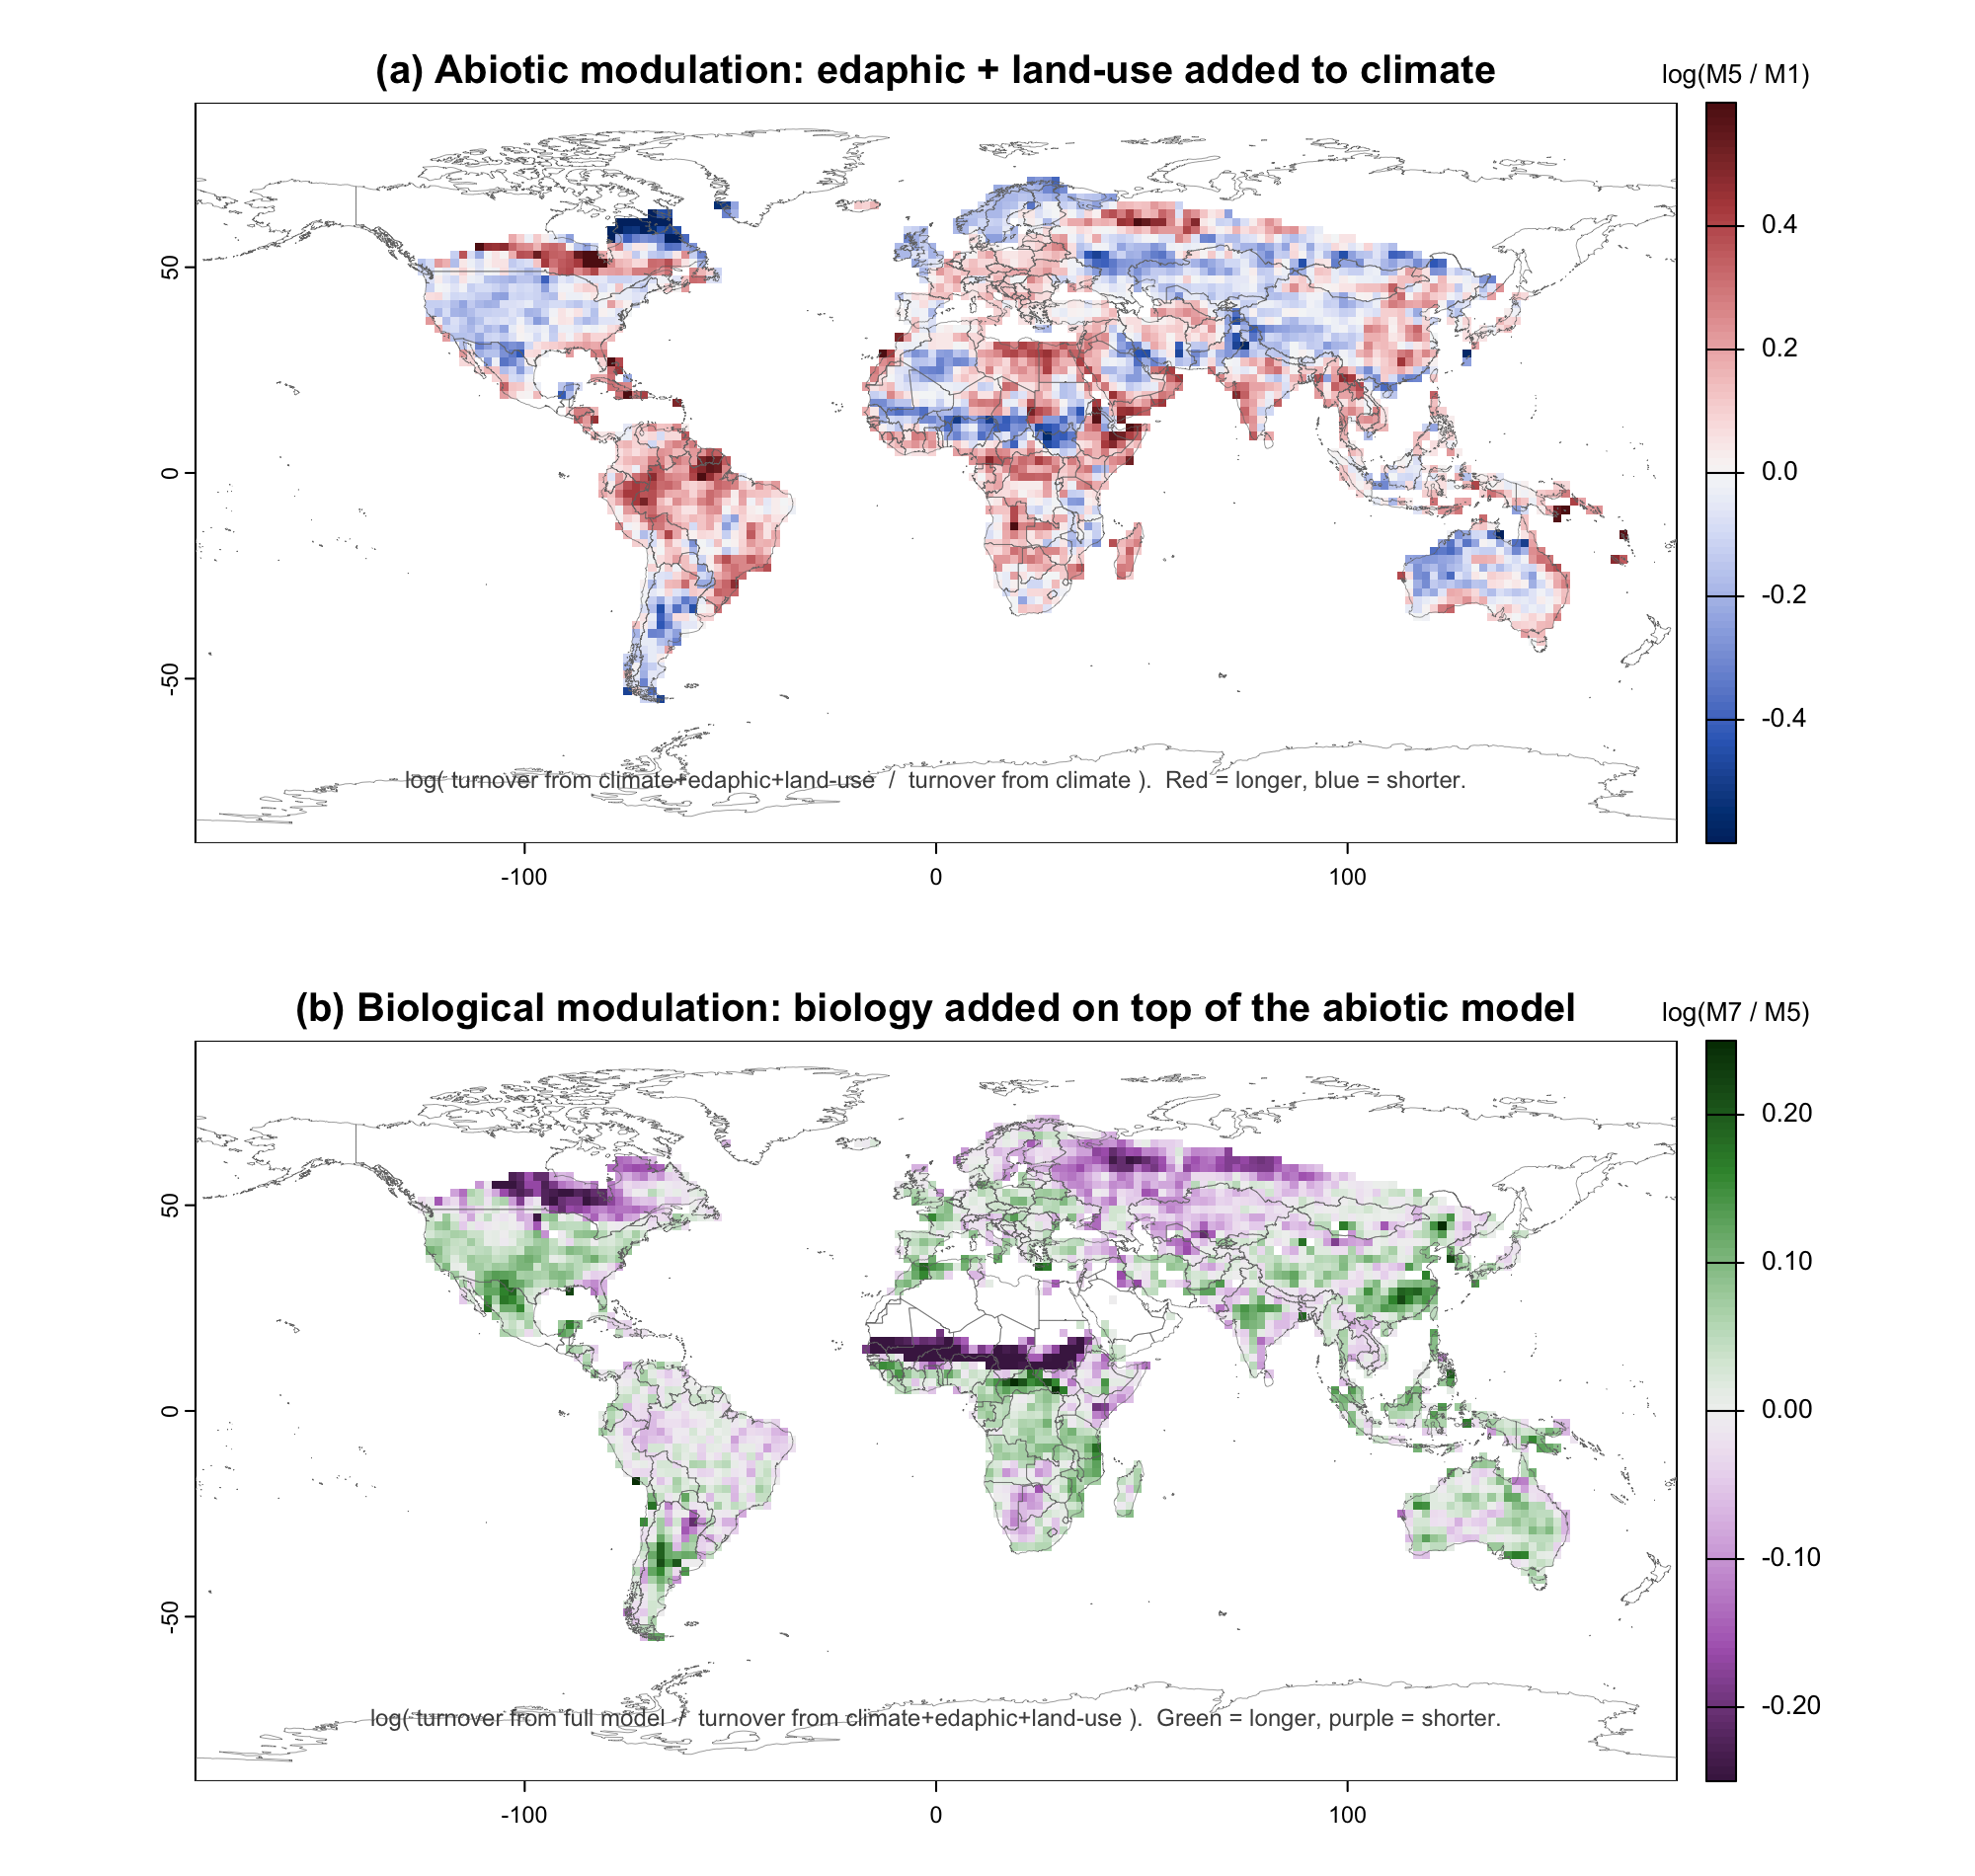
\includegraphics[width=0.8\textwidth]{../plots/step_15b_zonality/zonality_map_dual.png}
\caption{\textbf{Zonality map (nested).} The two domains taken sequentially rather than
symmetrically: (a)~abiotic modulation relative to climate and (b)~biological modulation
added on top of the abiotic model (order-dependent), at meso ($2\textdegree$) scale.
Red/green~=~longer turnover, blue/purple~=~shorter.}
\label{sfig:nestedmap}
\end{figure}

\begin{figure}[H]\centering
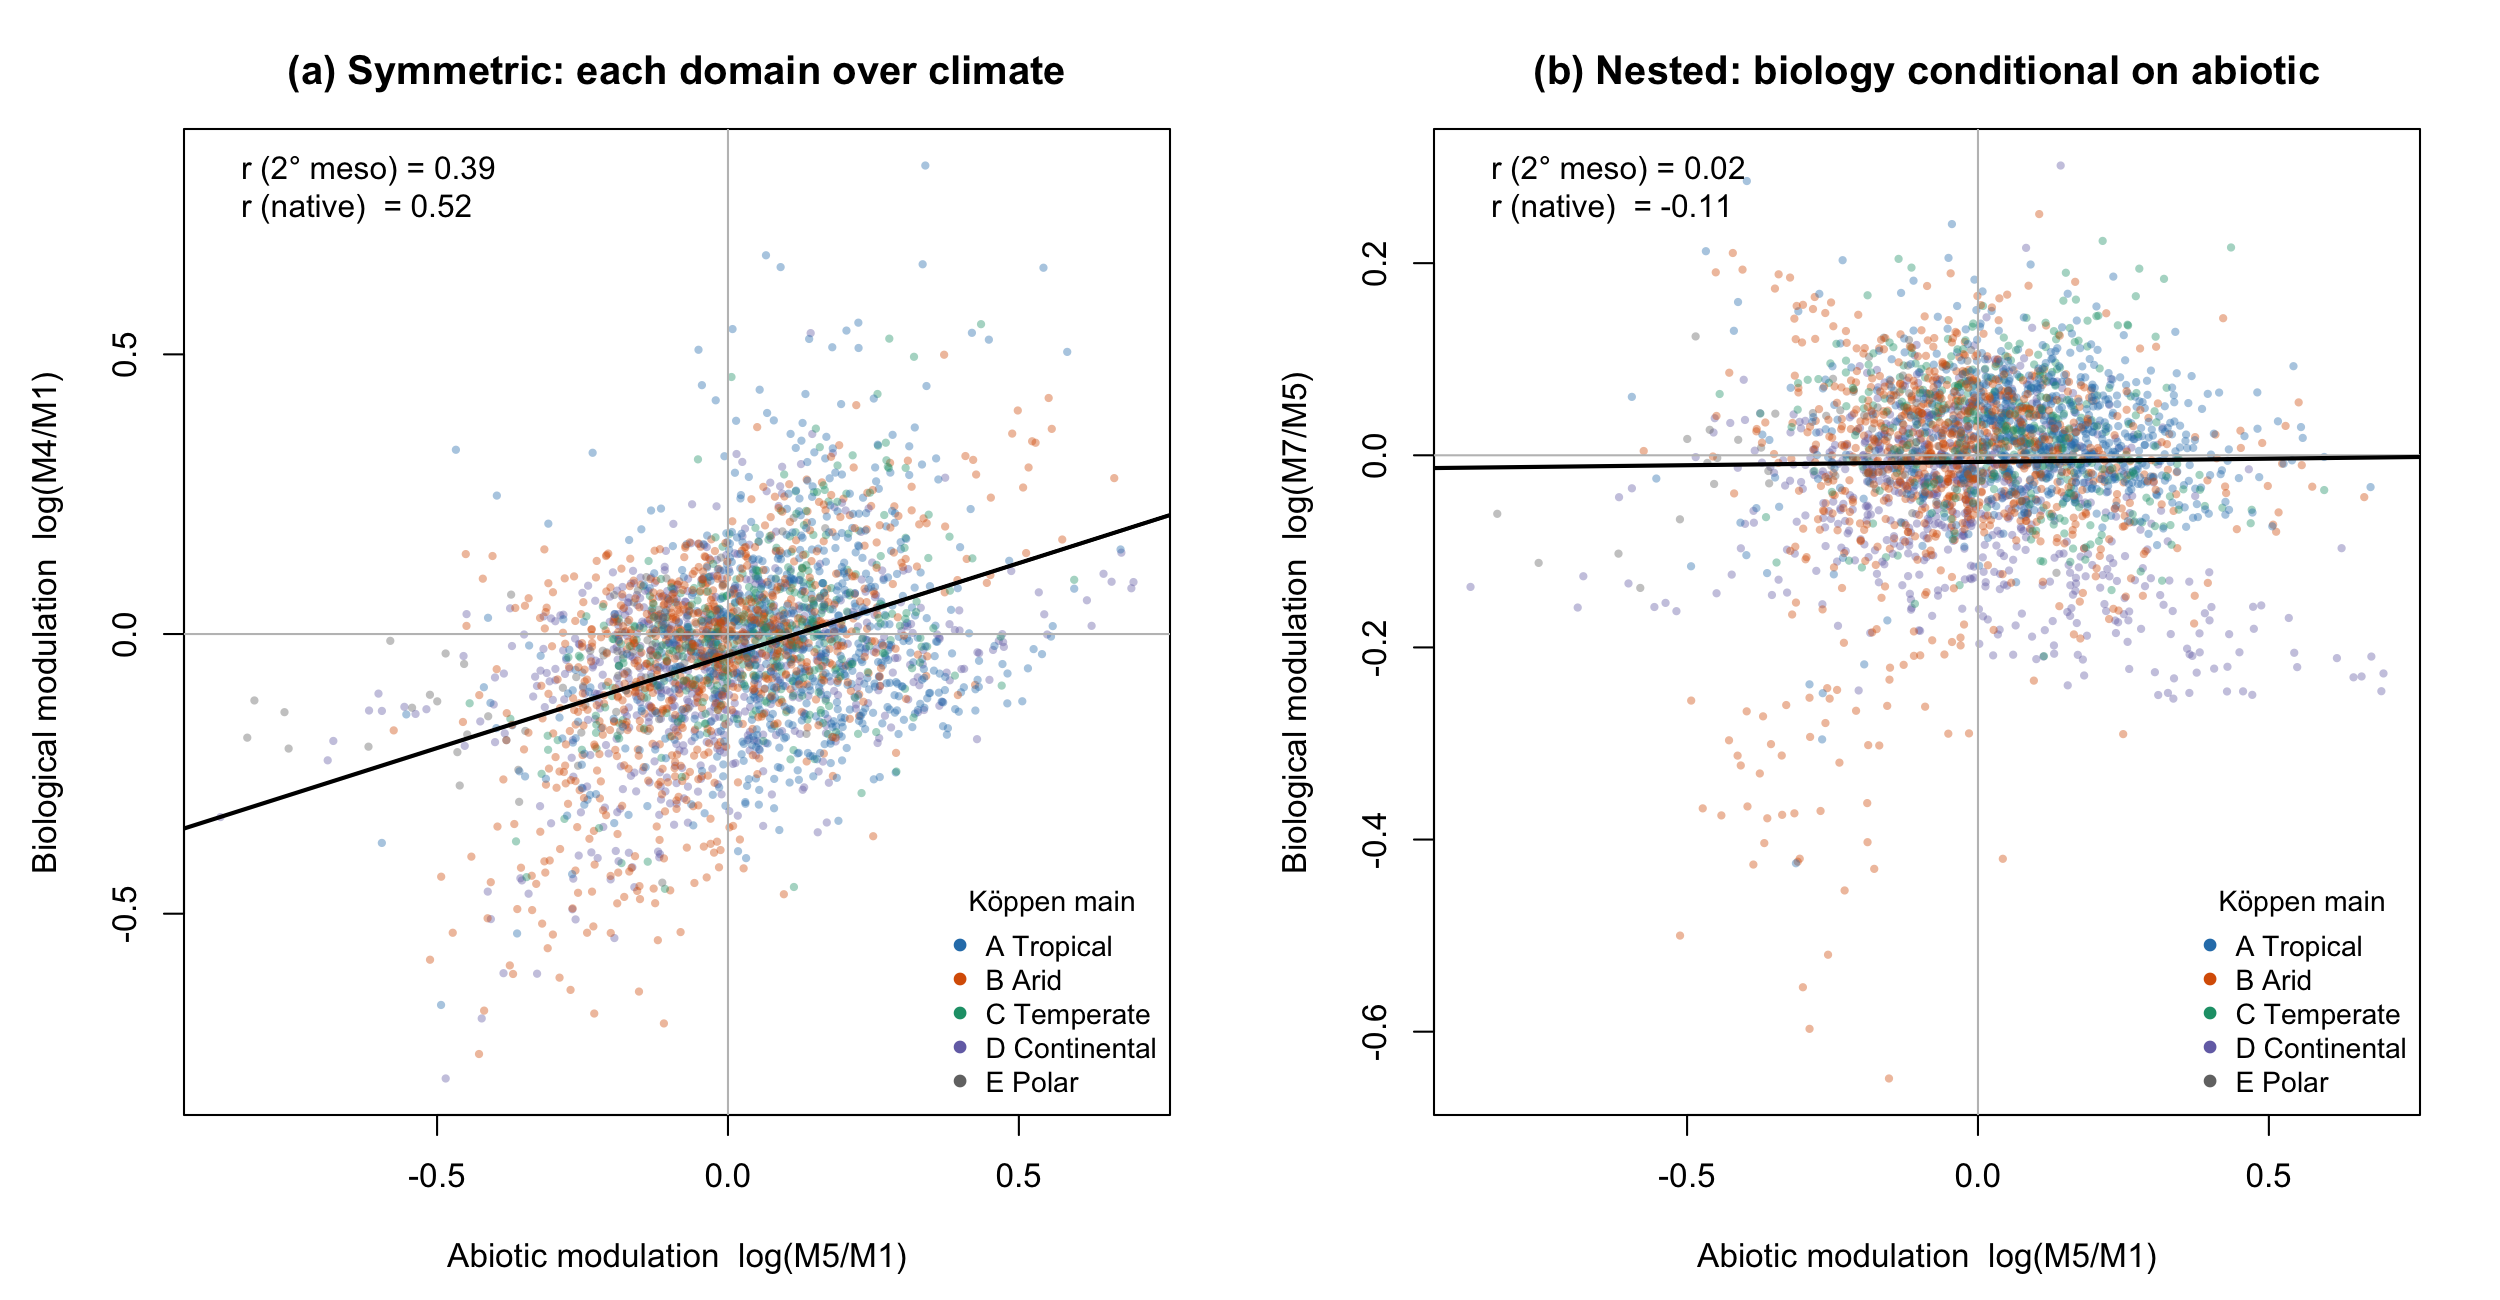
\includegraphics[width=0.72\textwidth]{../plots/step_15b_zonality/zonality_modulation_scatter.png}
\caption{\textbf{Abiotic versus biological modulation} (K\"oppen-coloured): the
symmetric pair co-varies ($r\approx0.4$--0.5) through the shared climate backbone, while
the nested pair is orthogonal ($r\approx0$), showing soil biology as a distinct axis.}
\label{sfig:bioscatter}
\end{figure}

\begin{figure}[H]\centering
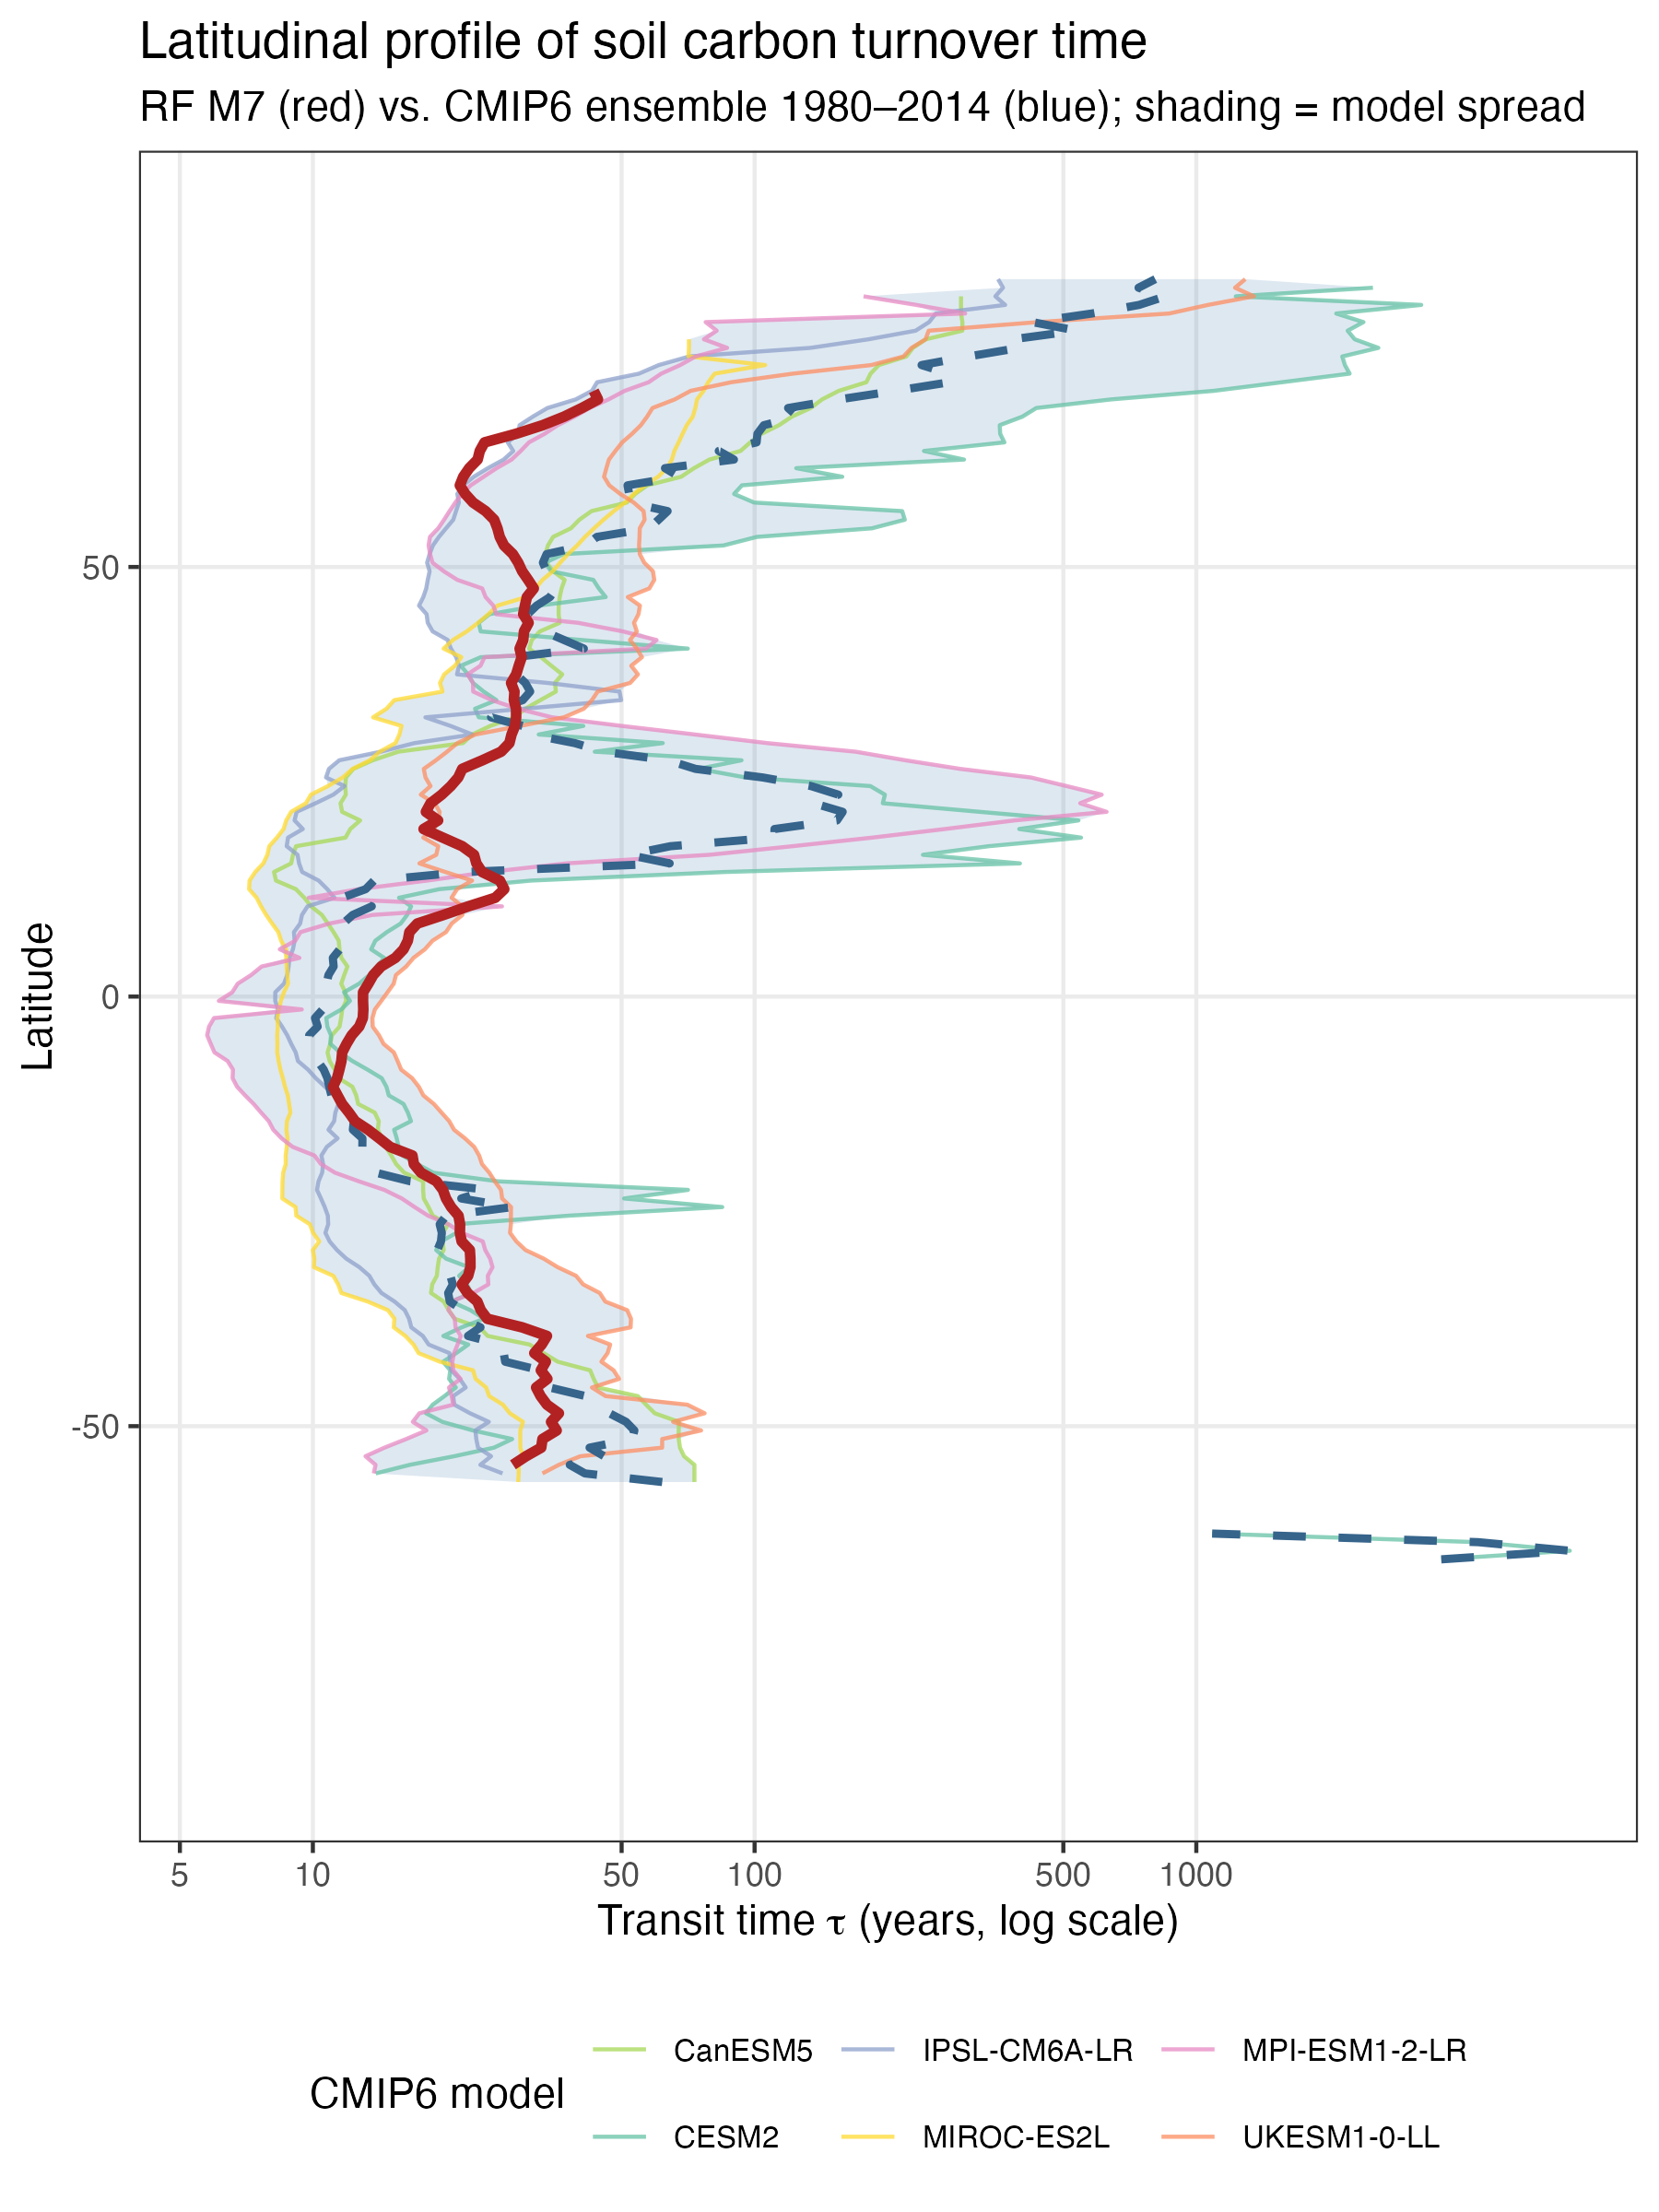
\includegraphics[width=0.7\textwidth]{../plots/step_20/fig_latitudinal_profile.png}
\caption{\textbf{Absolute latitudinal profile} of $\tau$ (log axis): CMIP6 members,
ensemble mean, and RF~M7. The magnitude counterpart to the normalised comparison in the
article; absolute values are not compared across products.}
\label{sfig:esm_profile}
\end{figure}

% =============================================================================
\section{Supplementary Tables}
% =============================================================================

\begin{table}[h!]
  \centering\small
  \caption{\textbf{Provenance control.} Coarse-scale organisation of the beyond-climate
  residual (ratio of observed between-block variance to the spatial-randomness null) and
  covariate skill on the block-mean residual, before and after removing each source
  database's mean. The signal is essentially unchanged, indicating it is ecological
  rather than a source/laboratory artefact.}
  \label{stab:provenance}
  \begin{tabular}{lcc}
    \toprule
    Metric & Before & After source de-meaning \\
    \midrule
    Between-source variance share ($\eta^2_\text{source}$) & \multicolumn{2}{c}{0.024 (2.4\,\%)} \\
    Organisation @\,2\textdegree{} (obs/null)   & $5.3\times$  & $5.1\times$ \\
    Organisation @\,5\textdegree{} (obs/null)   & $7.2\times$  & $6.4\times$ \\
    Organisation @\,10\textdegree{} (obs/null)  & $11.6\times$ & $10.1\times$ \\
    Block-mean covariate $R^2$ @\,5\textdegree{} & 0.188 & 0.152 \\
    \bottomrule
  \end{tabular}
\end{table}

\begin{table}[h!]
  \centering\small
  \caption{\textbf{Belowground NPP allocation fractions ($f_\text{BNPP}$)} by dominant
  land-cover class, used to estimate soil carbon input.}
  \label{stab:allocation}
  \begin{tabular}{lcc}
    \toprule
    Land cover class & ESA code & $f_\text{BNPP}$ \\
    \midrule
    Tree cover & 10 & 0.35 \\
    Shrubland & 20 & 0.45 \\
    Grassland & 30 & 0.55 \\
    Cropland & 40 & 0.30 \\
    Built-up & 50 & 0.20 \\
    Bare/sparse & 60 & 0.30 \\
    Herbaceous wetland & 90 & 0.50 \\
    Mangroves & 95 & 0.40 \\
    Moss/lichen & 100 & 0.60 \\
    \midrule
    \textit{Default (missing)} & --- & 0.40 \\
    \bottomrule
  \end{tabular}
\end{table}

\begin{table}[h!]
  \centering\small
  \caption{\textbf{Magnitude-free measures of spatial dispersion in $\tau$ across
  products.} Computed over all valid land pixels on the common $1\textdegree$ grid.
  CV~=~coefficient of variation; $\tau_{95}/\tau_{5}$~=~95th/5th percentile ratio;
  SD$_{\ln\tau}$~=~standard deviation of $\ln\tau$.}
  \label{stab:esm_dispersion}
  \begin{tabular}{llcccc}
    \toprule
    Product & LSM & Mean $\tau$ (yr) & CV & $\tau_{95}/\tau_{5}$ & SD$_{\ln\tau}$ \\
    \midrule
    CESM2 & CLM5 & 193.8 & 3.64 & 112.0 & 1.38 \\
    UKESM1-0-LL & JULES & 63.3 & 3.09 & 10.0 & 0.82 \\
    IPSL-CM6A-LR & ORCHIDEE & 27.5 & 2.02 & 6.3 & 0.74 \\
    MPI-ESM1-2-LR & JSBACH & 62.8 & 3.48 & 40.2 & 1.10 \\
    CanESM5 & CLASS-CTEM & 48.6 & 1.32 & 26.1 & 1.05 \\
    MIROC-ES2L & VISIT-e & 31.4 & 0.90 & 10.7 & 0.89 \\
    \midrule
    RF~M7 (this study) & --- & 23.2 & 0.39 & 3.7 & 0.42 \\
    \bottomrule
  \end{tabular}
\end{table}

% =============================================================================
\bibliographystyle{apalike}
\bibliography{references}
% =============================================================================

\end{document}
